\documentclass[a4paper, 12pt]{article}

\usepackage[utf8]{inputenc}
\usepackage[T1]{fontenc}
\usepackage[french]{babel} 
\usepackage[top=35mm, bottom=35mm, left=25mm, right=25mm]{geometry}
\usepackage{geometry}
\usepackage{graphicx}
\usepackage{multirow}  
\usepackage{subfigure}
\usepackage{verbatim}
\usepackage{url}
\usepackage{algorithmic, algorithm} 
\usepackage{amsmath,amsfonts,amssymb}
\usepackage{lmodern}
\usepackage{microtype}
\usepackage{xcolor}
\usepackage{textcomp}
\usepackage{minted}
\usepackage{framed}
\usepackage{tcolorbox}
\usepackage{etoolbox}
\BeforeBeginEnvironment{minted}{\begin{tcolorbox}[left=8mm]\begin{center}}
\AfterEndEnvironment{minted}{\end{center}\end{tcolorbox}}%
\usepackage{hyperref}
\hypersetup{
    colorlinks,
    citecolor=blue,
    filecolor=black,
    linkcolor=magenta,
    urlcolor=blue,
}
\hypersetup{
pdfpagemode={},
pdfstartview={XYZ 3000 3000 0.75}
pdfstartview={XYZ left top zoom}
}
\hypersetup{
pdftitle={Template de rapport \LaTeX},
pdfsubject={Sujet du rapport, peut être vide},
pdfauthor={Premier auteur et Deuxième auteur},
pdfkeywords = {Premier mot clé, Deuxième mot clé, etc...}
}
\setcounter{secnumdepth}{3}
\usepackage{fancyhdr}
\pagestyle{fancy}
 \lhead{\leftmark}
 \rhead{}
\usepackage{pgf, tikz}
\usetikzlibrary{arrows}


\newcommand{\makelogos}{
\begin{tikzpicture}[remember picture,overlay]
\node [shift={(3 cm,-2cm)}]  at (current page.north west){

\includegraphics[scale=.25]{images/insacvl.png}
};
\node [shift={(-3.675 cm,-2cm)}]  at (current page.north east){
\begin{minipage}{.01\textwidth}
\rotatebox{90}{\scalebox{.75}{Département}~~~~}
\end{minipage}
};
\node [shift={(-3 cm,-2cm)}]  at (current page.north east){
\begin{minipage}{.1\textwidth}
\hspace{-.5cm}
\begin{eqnarray}
&\textbf{{\color{red}S}}&\!\!\!\!\!\textnormal{écurité et}\nonumber\\
&\textbf{{\color{red}T}}&\!\!\!\!\!\textnormal{echnologies}\nonumber\\
&\textbf{{\color{red}I}}&\!\!\!\!\!\!\textnormal{nformatiques}\nonumber
\end{eqnarray}
\end{minipage}
};
\end{tikzpicture}
}
 % A priori, vous n'aurez pas besoin de modifier le contenu de ce fichier :)

\begin{document}
\pagenumbering{roman} 

%%% Remarque sur la page de garde :
% Il existe une commande beaucoup plus simple : \maketitle
% Cette commande ne permet pas directement l'insertion de logo et de données 
% additionnelles sans modifier certains fichiers de configuration
% (utilisation avancée)

\begin{titlepage}
\setlength{\headheight}{0cm}
\setlength{\headsep}{0cm}
{

%%% Insertion des logos [begin]
\makelogos
%%% Insertion des logos [end]

\vspace{4cm}

\begin{center}
\fbox{ 
\begin{minipage}[h]{.9\linewidth}
\begin{center}
{\vspace*{5mm}
\huge\textbf{Rapport Ouverture Scientifique et Technique}\\  %%% Titre du rapport
\vspace*{5mm}}
\end{center}
\end{minipage}
}

\vspace{15mm}

Auteur\\~\\
{\large 
\bsc{Dubois} Louan\\
\bsc{Maachi} Kaoutar\\
\bsc{Techer} Luc}\\
~\\
\underline{STI, 4A}\\ 

\vspace{3cm}  

\textbf{Année Universitaire 2020 - 2021\\
{\tiny version : \today}}

\vspace{2cm}  

\end{center}
  
\vfill

\begin{flushleft}
	Encadrant : \textsc{Toinard} Christian
\end{flushleft}

}
\end{titlepage}

\newpage		
\tableofcontents % Insertion de la table des matières
\addcontentsline{toc}{section}{Table des matières}

% Vous pouvez également pour des rapports plus longs (des rapports de stages par exemple) insérer une table des figures
%\listoffigures
%\addcontentsline{toc}{section}{Liste des figures} 

% Voir même une liste des algorithmes
%\listofalgorithms
%\addcontentsline{toc}{section}{Liste des algorithmes}

\clearpage 

\pagenumbering{arabic} 
\section{Contexte}
Un système d'exploitation est principalement composé d'un noyau. Celui-ci est une couche d'abstraction entre le matériel (processeur, mémoire) et le logiciel (application, \emph{user space}), et permet leur communication. Il peut être monolithique, c'est-à-dire un programme qui est tel qu'il est et ne peut pas être modifié, pas d'ajout de fonctionnalités possible sans le recompiler. Il peut également être modulaire, qui signifie que l'on peut lui ajouter des programmes qui étendent ses fonctionnalités, et aussi les supprimer. 

Voici une première section. Vous pouvez faire des citations en utilisant la commande \textbackslash\texttt{cite}. Par exemple \cite{DH76}.

Les informations de publication concernant le papier cité sont à placer dans un fichier \texttt{.bib}. Dans ce template, il s'agit du fichier \texttt{bibliographie.bib}.

Ces informations peuvent être obtenues sur le web, notamment ici : 
\begin{center}
\url{https://scholar.google.fr/}
\end{center}


Pour ce faire :
\begin{enumerate}
\item chercher le nom de l'article,
\item cliquez sur les guillemets,
\item puis sur BibTeX,
\item copier l'intégralité du texte dans le fichier \texttt{bibliographie.bib},
\item modifier la clé,
\item dans votre fichier \texttt{rapport.tex}, utilisez cette clé pour citer le papier.
\end{enumerate} 

\underline{Exemple :} New directions in Cryptography, de Diffie et Hellman

\begin{enumerate}
\item La recherche : \url{https://scholar.google.fr/scholar?hl=fr&as_sdt=0%2C5&q=new+directions+in+cryptography&btnG=&oq=New+directions+in+cryptography}
\item L'entrée BibTeX : \url{https://scholar.googleusercontent.com/scholar.bib?q=info:zhumlNGssTEJ:scholar.google.com/&output=citation&scisig=AAGBfm0AAAAAXJH2ZyWHII7hxbyh6hti-poxCXmdN6Bc&scisf=4&ct=citation&cd=-1&hl=fr&scfhb=1}
\item Ici, la clé par défaut est \texttt{diffie1976new}, que je modifie en \texttt{DH76}. 
\item Pour citer ce papier, dans \texttt{rapport.tex}, j'utilise la commande \textbackslash\texttt{cite}\{\texttt{DH76}\}
\end{enumerate}



Vous pouvez aussi mettre des références en URL en pied de page\footnote{Il suffit d'utiliser la commande \textbackslash\texttt{footnote} et d'inclure votre URL à l'aide de \textbackslash\texttt{footnote} : \url{https://www.latex-project.org/} ou de \textbackslash\texttt{href} : \href{https://www.latex-project.org/}{même lien}.} (mais c'est moins propre que \textbackslash\texttt{cite}).
 

Attention, les compilations \LaTeX et BibTeX peuvent être... ``capricieuses''. Je vous recommande de suivre cet ordre :
\begin{enumerate}
\item Compilation \LaTeX{} : \texttt{pdflatex -synctex=1 --shell-escape -interaction=nonstopmode rapport.tex}
\item Compilation BibTeX : \texttt{bibtex rapport.aux}
\item Compilation \LaTeX{}
\item Compilation \LaTeX{}
\end{enumerate}
Ou plus simplement, utilisez le \texttt{Makefile} fourni.

\clearpage 
\section{Problématique}

Dans les années 1990, tous les systèmes d'exploitation étaient basés sur des noyaux monolithiques ce qui limitait grandement les possibilités de développement de systèmes en rendant compliqué l'intégration de tels noyaux sur des architectures matérielles complexes. Les développeurs avaient alors besoin d'un système d'exploitation fiable, sécurisé et modulable afin de pouvoir l'exploiter au mieux dans leurs applications. \\
De plus, un noyau monolithique limite la compatibilité et l'optimisation vis-à-vis d'architectures variées. A l'époque, les ordinateurs hautes performances et les super-ordinateurs possaidaient plusieurs processeurs tandis que les ordinateurs grand-public n'en possaidaient qu'un. L'objectif de cette recherche était donc de créer un noyau modulaire qui pouvait être facilement adapté à différentes architectures plus ou moins complexes.

\subsection{Une première sous-partie}
\paragraph{}
Un premier paragraphe...
\paragraph{}
Un second...

\subsection{Une seconde sous-partie}
\paragraph{Inclusion d'images/screenshot} \textcolor{blue}{$\leftarrow$ on peut donner des titres aux paragraphes :)} 

Dans ce paragraphe, on va inclure une petite image (centrée) :

\begin{figure}[h]
\centering
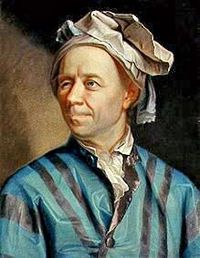
\includegraphics[scale=.5]{images/euler.jpg}
\caption{\label{euler}Avec une légende :)}
\end{figure}

Et plus loin on peut même faire (et simplement) référence à la Figure \ref{euler} page \pageref{euler}.

Les formules de maths sont entre \$ comme ceci $\exp^{i\pi} + 1 = 0$ ou encore entre \$\$ pour les centrer : $$\sum_{n=1}^{+\infty} \frac{1}{n^2} = \frac{\pi^2}{6}.$$

On peut également utiliser un environnement dédié :

\begin{equation}
\label{eq:zsurpz}
\mathbb{Z}/p\mathbb{Z} = \left\lbrace 0, 1, \ldots, p-1  \right\rbrace
\end{equation}

Et même aligner les équations simplement et proprement avec un autre environnement :

\begin{eqnarray}
t &=& a+b+c\\
&=& d+e \\
&=& z^{x\times y}\label{eq:ici}\\
&=& \left(\frac{\delta + \omega}{\tau}\right)
\end{eqnarray}

Et faire références à ces équations \eqref{eq:zsurpz} et \eqref{eq:ici}.

\clearpage 
\section{Apports scientifiques principaux de l’article}
\subsection{Le concept des micro-noyaux}
\paragraph{}

Dans cet article, le concept des micro-noyaux est introduit. Il s'agit d'une solution qui consiste à réduire au plus possible le noyau (aussi appelé Nucleus) afin que celui-ci ne puisse effectuer que des tâches élémentaires. Les autres fonctionnalités seront quant à elles effectuées par des serveurs modulaires. Ces serveurs sont en réalité des sous-systèmes qui pourront échanger des informations entre-eux en utilisant des Communications Inter-Processus (IPC). Ces différents sous-systèmes pourront alors être répartis sur un seul ou plusieurs processeurs ou machines. Afin de faciliter les communications entre les différents serveurs, l'article propose aussi la mise en place de Remote Procedure Call (RPC) qui est un protocole qui permet d'exécuter des commandes sur un serveur à distance. \\
La mise en place de micro-noyaux permettrait de faciliter grandement la répartition et l'isolations de différentes parties du systèmes sur des processeurs ou machines différentes tout en restant compatible avec des architectures plus simples. Ceci permettrait aussi aux développeur de pouvoir créer, tester et implémenter de nouvelles fonctionnalités beaucoup plus simplement.

\subsection{Présentation de Chorus}


\clearpage 
\section{Impacts de l'article}

\clearpage 
\section{Analyse critique du travail proposé}

\clearpage 
\section*{Conclusion}
\addcontentsline{toc}{section}{Conclusion}

Ce magnifique projet nous a permis -- outre de nous familiariser avec \LaTeX{} -- de \ldots

\clearpage 
\bibliographystyle{plain}
\bibliography{bibliographie}
\addcontentsline{toc}{section}{Références}


\clearpage 
\appendix
\bigskip\noindent{\Large\bf Annexes}
\addcontentsline{toc}{section}{Annexes}
\section{Algorithme qui fait quelque chose}
\begin{minted}{c}
#include<stdio.h>

int main()
{
	printf("Hello World !\n);
	return 0;
}
\end{minted}

\clearpage 
\section{Une autre annexe}

\end{document}
